
\section{Theoretical background of the models}

Here we review the mathematical background of the models we have used fot this project. We will mainly follow  \cite{lindholm2022machine}.

    %%%%%%%%%%%%%%%%%%%%%%%%%%%%%%%%
    %%%%%%%%%%%%%%%%%%%%%%%%%%%%%%%%
    %%%%%%%%%%%%%%%%%%%%%%%%%%%%%%%%
    %%%%%%%%%%%%%%%%%%%%%%%%%%%%%%%%
    %%%%%%%%%%%%%%%%%%%%%%%%%%%%%%%%
    \subsection{Logistic Regression}
    The backbone of the \emph{logistic regression} is linear regression, i.e. finding the least-squares solution to an equation system 
        \begin{equation*}
            X\theta = y,
        \end{equation*}
     where $X$ is the training data matrix, $\theta$ is the coefficient vector (also called parameter vector), and $y$ is the training output. The solution to the system above is given by the normal system of equations 
        \begin{equation*}
            X^TX \theta = X^Ty
        \end{equation*}
    The parameter vector $\theta$ is then used in the sigmoid function $\sigma(z): \mathbb{R}\to [0,1]$
    \begin{equation*}
        \sigma(z) = \frac{e^{z}}{1+e^{z}}
    \end{equation*}
    where $  z = x^T \theta$, and $x$ is the testing input. This gives a statistical interpretation of the input vector, meaning $\sigma(z)$ maps the linear combination $z$ to a probability value in the interval $[0,1]$. In the case of a binary True/False classification, the value of the sigmoid function  determines the class. The model was tuned using the \texttt{lbfgs} algorithm, which is standard in \emph{SKLearn}. It optimizes the weights  $\theta_i$ to minimize the log-loss function, defined by 
    \begin{equation}
        J(\theta) = - \frac{1}{m} \sum_{i=1}^{m} \left[ y_i \log(h_\theta(x_i)) + (1 - y_i) \log(1 - h_\theta(x_i)) \right] + \frac{\lambda}{2} ||\theta||^2,
    \end{equation}
    where $\lambda$ is the regularization strength (default for SKLearn is $\lambda = 1.0$), $h_\theta$ is the sigmoid function for each of the $m$ input vectors $x_i$, and $\theta$ is the parameter vector that will be optimized. For the optimization we have used a gradient method.

    
    %%%%%%%%%%%%%%%%%%%%%%%%%%%%%%%%
    %%%%%%%%%%%%%%%%%%%%%%%%%%%%%%%%
    %%%%%%%%%%%%%%%%%%%%%%%%%%%%%%%%
    %%%%%%%%%%%%%%%%%%%%%%%%%%%%%%%%
    %%%%%%%%%%%%%%%%%%%%%%%%%%%%%%%%
    \subsection{Random forest}
    %These divisions are then used to create a binary tree shown in figure \ref(Tree) ingen figur, så tar bort det.
    
    The \emph{random forest method} is  based on so called decision trees, i.e. the data points are divided into binary groups based on Gini-impurity, entropy or classification error. Gini-impurity is the most commonly used. These divisions are then used to create a binary tree, where the thee leaf-nodes are used to classify the target variables, based on the input.
    
    The division tree itself usually gives unsatisfying results, which leads to developing methods such as random \emph{forest} and \emph{sandbagging}. These methods are considered to be more accurate.
    
    Sandbagging is a technique that samples the given data multiple times, in order to create multiple data sets extracted from the original data set. In the next a decision tree model is trained on each sample-subset, and the prediction of each sample-subset is then combined into one model. 
    
    This decreases the variance of the model, but at the same time increases bias, which means that sandbagging can increase false negatives, hence the model is non-viable for our project.
    
    On the other hand, random forest is viable, since it creates multiple trees, meanwhile it disregards the random input variable. The randomness of the process results in decreased overfitting, and we therefore have a more robust model.
    
 
    
    %%%%%%%%%%%%%%%%%%%%%%%%%%%%%%%%
    %%%%%%%%%%%%%%%%%%%%%%%%%%%%%%%%
    %%%%%%%%%%%%%%%%%%%%%%%%%%%%%%%%
    %%%%%%%%%%%%%%%%%%%%%%%%%%%%%%%%
    %%%%%%%%%%%%%%%%%%%%%%%%%%%%%%%%
    \subsubsection{Non-parametric method: k--Nearest Neighbour}
    Let $\{ \boldsymbol{x}_i, y_i \}_{n \in \mathbb{N}}$ be the training data set, where $\boldsymbol{x_i}$ is a matrix representing the input, and $y_i$ is the  output.
    
    \emph{$k$-- Nearest Neighbour}($k$--NN) is a distance based method that takes a $k$ amount of points from the training data set, called \emph{neighbours}, computes the distance between them, then assumes that the predicted value $\hat{y}(x_{*})$ follows the trend of the $k$-- nearest neighbours. Since $k$--NN uses the training data explicitly it is also called a \emph{nonparametric} method.

    The $k$--NN method can be divided into several subcategories, inter alias \emph{classification} $k$--NN method, \emph{regression}  $k$--NN method. In this project, we are using the classification method, since we are trying to predict in which of the two classes low, or high demand, the given, and predicted data points belong.

    The classification  $k$--NN algorithm evaluates $\hat{y}(x_{*})$ by computing the most frequently occurring class among the $k$ nearest neighbours. Here, we try to identify whether a data point belong to the high demand-class. Denote $c=$ high demand class. For simplicity, assume Euclidean ambiance. Then
        \begin{equation*}
            \hat{y}(x_*) = \arg \max_{c}  \sum_{n \in \mathbb{N}} \chi_{(y_i = c)} ,
        \end{equation*}
    where $y_i$ is the class of the nearest neighbour,  $\chi$ is the characteristic function 
        \begin{equation*}
            \chi_{(y_i = c)} = 
            \begin{cases}
                1 \qquad \text{if } y_n = c, \\
                0 \qquad \text{otherwise}.
                
            \end{cases}
        \end{equation*}
    It is very common to use a weighted sum to predict the next value, i.e.
        \begin{equation*}
            \hat{y}(x_*) =  arg \max_{c}  \sum_{n \in \mathbb{N}} \frac{\chi_{(y_n = c)}}{d(x, x_n)},
        \end{equation*}
    where $d$ is the standard Euclidean metric, computing the distance between an input $x$, and a neighbour $x_n$. 

    When using this model it is important to choose an optimal $k$--value. There are several tests for this, here we implement \emph{uniform weighting}, and \emph{distance weighting}. The first algorithm creates a $k$--NN model for each new $k \in [1, 500]$, and trains the model with uniform weights, i.e. the contribution of all neighbours is equal. Similarly, the latter trains a $k$--NN classifier for each $k \in [1, 500]$, with the difference that it uses distance based weighting, i.e. closer neighbours have greater influence. After testing different upper boundaries for $k$, the two models gave good results in the interval $[1,500]$, see Figure \ref{fig:kNN_comparison}. From the figures, we can see that the second test gives a better value for $k$, since the plot follows smoother trend, in comparison to the uniform weighting test, which makes it easier to identify an optimal $k$ value ($k = 120$). Moreover, the distance weighting algorithm is providing results for larger values of $k$, that is for $k \in [1, 400)$ before the curve converges, while the uniform weighting algorithm converges earlier, when $k = 120$. This means that for large $k$, both test algorithms make prediction based on the most common class in the data set, instead of making prediction based on the behaviour of the neighbours. Thus for sufficiently large $k$, for any given data point, the model will consider unnecessarily large amount of neighbours, and the prediction will be evaluated to belong to the most frequent class. Since the distance weighting has a larger range of $k$--value, it should be more trustworthy.

    When $k = 120$, the accuracy of the model is 92\%.
    
    \begin{figure}[htbp]
        \centering
        \begin{subfigure}{0.45\textwidth}
            \centering
            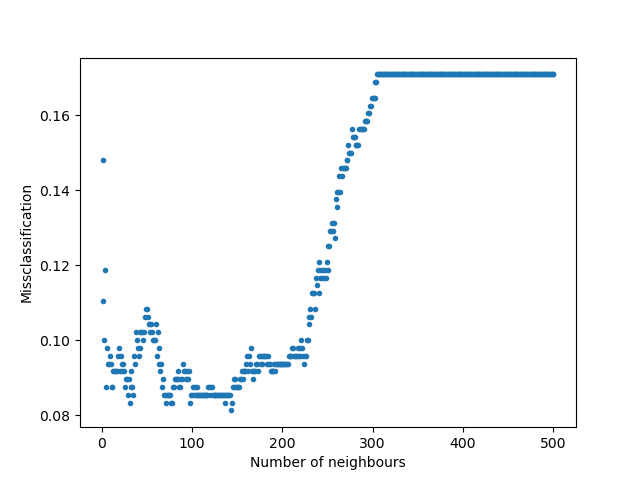
\includegraphics[width=\textwidth]{NYkNNtest1.png}
            \caption{Uniform distance test for $k$.}
            \label{fig:kNN_fig1}
        \end{subfigure}
        \hfill
        \begin{subfigure}{0.45\textwidth}
            \centering
            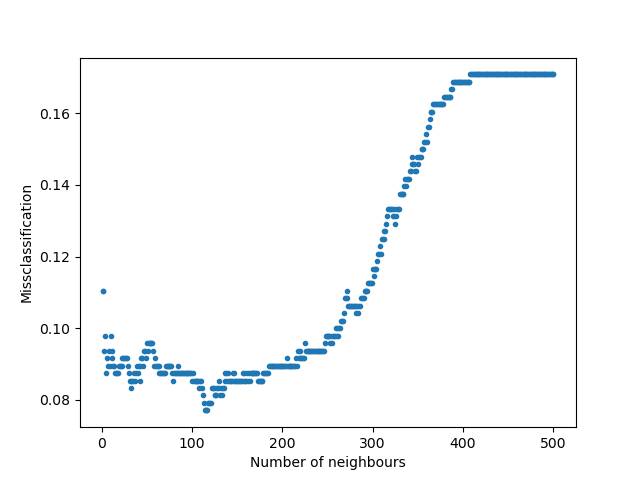
\includegraphics[width=\textwidth]{NYkNNtest2.png}
            \caption{Weighted distance test for $k$.}
            \label{fig:kNN_fig2}
        \end{subfigure}
        \caption{Test for choosing an optimal $k$--value.}
        \label{fig:kNN_comparison}
    \end{figure}

    

    %%%%%%%%%%%%%%%%%%%%%%%%%%%%%%%%
    %%%%%%%%%%%%%%%%%%%%%%%%%%%%%%%%
    %%%%%%%%%%%%%%%%%%%%%%%%%%%%%%%%
    %%%%%%%%%%%%%%%%%%%%%%%%%%%%%%%%
    %%%%%%%%%%%%%%%%%%%%%%%%%%%%%%%%   
    \newpage
    \subsection{Discriminant analysis: LDA and QDA}
    
    \emph{Linear Discriminant Analysis} is a generative model, which means it is a model that creates and uses a  priori probability 
    distribution $P(\mathbf{x}, y)$ to estimate the posterior probability $P(y=m|\mathbf{x})$.  Here $\mathbf{x}$ is a feature vector,  $y$ is a class label belonging to some specific class $m$. In other words we compute the conditional probability $P(y=m|\mathbf{x})$ by using  Bayes' theorem, which states
        \begin{equation*}
            P(y|\mathbf{x}) = \frac{P(y,\mathbf{x})}{P(\mathbf{x})} = \frac{P(y)P(\mathbf{x}|y)}{\int_y P(y,\mathbf{x})}.
        \end{equation*}
        
    When discrete variables are used, we have the following formulation of Bayes' theorem 
    \begin{equation*}
        p(y=m|\mathbf{x}) = \frac{p(y=m)p(\mathbf{x}|y=m)}{\sum_{m=1}^{M} p(y=m) p(\mathbf{x}|y=m)}.
    \end{equation*}
    %For this form of the equation to be useful, it is neccesary to obtain an accurate estimation of $p(y=m)$ and $p(\mathbf{x}|y=m)$
    for all classes m. 
    \\
    
    In LDA, $p(y=m)$ is estimated by calculating the proportion of the training data points of each class,  and then uses the calculated percentage as the probability of a certain data point belonging to a certain class. Mathematically
        \begin{equation*}
            p(y=m) = \frac{1}{n}\sum_{i=1}^{n}\mathbb{I}\{y_i=m\} = \frac{n_m}{n}
        \end{equation*}  

    We then use the multi-dimensional Gaussian distribution given by
        \begin{equation} \label{eq: Gaussiandistriburion LDA}
            \mathcal{N}(\mathbf{x}|\mathbf{\mu}, \mathbf{\Sigma}) = \frac{1}{(2 \pi)^{d/2} |\mathbf{\Sigma}|^{1/2}} 
            exp \left( -\frac{1}{2}(\mathbf{x}-\mathbf{\mu})^T \mathbf{\Sigma}^{-1} (\mathbf{x}-\mathbf{\mu})\right),
        \end{equation}
    in order to estimate the probability distribution $p(\mathbf{x}|y=m)$. In \eqref{eq: Gaussiandistriburion LDA}, $\mathbf{x}$ is the d-dimentional data point, $\mathbf{\mu}$ is the (d-dimentional) mean of the random variable,
    $\mathbf{\Sigma}$ is the symmetric, positive definite covariance matrix given by
        \begin{equation*}
            \mathbf{\Sigma} = \frac{1}{n-M}\sum_{m=1}^{M} \sum_{i:y_i=m} 
            (\mathbf{x}_i-\mathbf{\mu}_m)(\mathbf{x}_i-\mathbf{\mu}_m)^T.
        \end{equation*}
    Using the above estimations, we derive an expression for $p(y=m|\mathbf{x})$, for all $m$. By applying the maximum likelihood principle, LDA assigns $\mathbf{x}$ to the most probable class $m$. 
    
    Quadratic discriminant analysis (QDA) is based on LDA. The main difference is the computation of the covariance matrix $\mathbf{\Sigma}$. In LDA,  $\mathbf{\Sigma}$ is assumed to be the same for all classes. In QDA, $\mathbf{\Sigma}$ is computed for each class as follows
    \begin{equation*}
        \mathbf{\Sigma}_m = \frac{1}{n_m - 1} \sum_{i:y_i=m} 
        (\mathbf{x}_i-\mathbf{\mu}_m)(\mathbf{x}_i-\mathbf{\mu}_m)^T
    \end{equation*}
    
    To optimize LDA and QDA, we need to estimate $\mathbf{\Sigma}_m$ and $\mathbf{\mu_m}$ for all classes m. The mean $\mathbf{\mu}$ is given by the average of the input data $\mathbf{\mu} = \frac{1}{n_m}\sum_{i=1}^{n_m} \mathbf{x}_i$.

    Notice that both LDA, and QDA relay on a multi-variable Gaussian distribution, which is the best choice for normally distributed
    variables. However, in this project we are working with positive definite values, which usually are not normally distributed. This becomes problematic for the QDA model, because all data points of the class $\textit{high\_bike\_demand}$ have a
    snow depth of 0, hence no variance. As a result the inverse of the covariance matrix is not defined. To address this problem, we exclude this variable from this model. 
    

    %%%%%%%%%%%%%%%%%%%%%%%%%%%%%%%%
    %%%%%%%%%%%%%%%%%%%%%%%%%%%%%%%%
    %%%%%%%%%%%%%%%%%%%%%%%%%%%%%%%%
    %%%%%%%%%%%%%%%%%%%%%%%%%%%%%%%%
    %%%%%%%%%%%%%%%%%%%%%%%%%%%%%%%%
    \subsection{Input Data Modification}
    \label{sec:input data modification}
    By plotting the data and analyzing the .csv file, some observations were made. The different inputs were then changed accordingly:
    \begin{itemize}
        \item \emph{Kept as-is}: \texttt{weekday}, \texttt{windspeed}, \texttt{visibility}, \texttt{temp}
        \item \emph{Modified}:
        \begin{itemize}
            \item \texttt{month} - split into two inputs, one cosine and one sine part. This make the new inputs linear and can follow the fluctuations of the year. The original input was discarded.
            \item \texttt{hour\_of\_day} - split into three boolean variables: \texttt{demand\_day}, \texttt{demand\_evening}, and \texttt{demand\_night}, reflecting if the time was between 08-14, 15-19 or 20-07 respectively. This was done because plotting the data showed three different plateaues of demand for the different time intervals. The original input was discarded.
            \item \texttt{snowdepth}, \texttt{precip} were transformed into booleans, reflecting if it was raining or if there was snow on the ground or not. This was done as there was no times where demand was high when it was raining or when there was snow on the ground.
        \end{itemize} 
        \item \emph{Removed}: \texttt{cloudcover}, \texttt{day\_of\_week}, \texttt{snow}, \texttt{dew}, \texttt{holiday}, \texttt{summertime}. These were removed due to being redundant (e.g. \texttt{summertime}), not showing a clear trend (e.g. \texttt{cloudcover}), giving a worse score when used, or all three (e.g. \texttt{day\_of\_week}).
    \end{itemize}